\documentclass[14pt]{beamer}
%%%%%%%%%%%%%%%%%%%%%%%%%%%%%%%%%%%%%%%%%%%%%%%%%%%%%%%%%%%%%
% Meta informations:
\newcommand{\trauthor}{Daniel Speck und Florian Kock}
\newcommand{\trtype}{Praktikum} %{Proseminar} %{Seminar} %{Workshop}
\newcommand{\trcourse}{Neuronale Netze WS2014/15}
\newcommand{\trtitle}{Pong, gespielt von KNNs}
\newcommand{\tremail}{hansen@informatik.uni-hamburg.de}
\newcommand{\trinstitute}{Dept. Informatik -- Knowledge Technology, WTM}
\newcommand{\trwebsiteordate}{{}}

%%%%%%%%%%%%%%%%%%%%%%%%%%%%%%%%%%%%%%%%%%%%%%%%%%%%%%%%%%%%%
% Languages:

% Falls die Ausarbeitung in Deutsch erfolgt:
% \usepackage[german]{babel}
% \usepackage[T1]{fontenc}
% \usepackage[latin1]{inputenc}
% \usepackage[latin9]{inputenc}	 				
% \selectlanguage{german}

% If the thesis is written in English:
\usepackage[ngerman]{babel} 						
\selectlanguage{ngerman}



%%%%%%%%%%%%%%%%%%%%%%%%%%%%%%%%%%%%%%%%%%%%%%%%%%%%%%%%%%%%%
% Bind packages:
\usepackage{beamerthemesplit}
\usetheme{Boadilla}
%\usetheme{Copenhagen}
%\usetheme{Darmstadt}
%\usetheme{Frankfurt}
%\usetheme{Ilmenau}
%\usetheme{JuanLesPins}
%\usetheme{Madrid}
%\usetheme{Warsaw }
%\usecolortheme{dolphin}
%\setbeamertemplate{sections/subsections in toc}[sections numbered]
%\beamertemplatenavigationsymbolsempty
%\setbeamertemplate{headline}[default] 	% deaktiviert die Kopfzeile
\setbeamertemplate{navigation symbols}{}% deaktiviert Navigationssymbole
%\useinnertheme{rounded}

\usepackage{acronym}                    % Acronyms
\usepackage{algorithmic}								% Algorithms and Pseudocode
\usepackage{algorithm}									% Algorithms and Pseudocode
\usepackage{amsfonts}                   % AMS Math Packet (Fonts)
\usepackage{amsmath}                    % AMS Math Packet
\usepackage{amssymb}                    % Additional mathematical symbols
\usepackage{amsthm}
\usepackage{color}                      % Enables defining of colors via \definecolor
\usepackage{fancybox}                   % Gleichungen einrahmen
\usepackage{fancyhdr}										% Paket zur schickeren der Gestaltung der 
\usepackage{graphicx}                   % Inclusion of graphics
%\usepackage{latexsym}                  % Special symbols
\usepackage{longtable}									% Allow tables over several parges
\usepackage{listings}                   % Nicer source code listings
\usepackage{lmodern}
\usepackage{multicol}										% Content of a table over several columns
\usepackage{multirow}										% Content of a table over several rows
\usepackage{rotating}										% Alows to rotate text and objects
\usepackage[section]{placeins}          % Ermoeglich \Floatbarrier fuer Gleitobj. 
\usepackage[hang]{subfigure}            % Allows to use multiple (partial) figures in a fig
%\usepackage[font=footnotesize,labelfont=rm]{subfig}	% Pictures in a floating environment
\usepackage{tabularx}										% Tables with fixed width but variable rows
\usepackage{url,xspace,boxedminipage}   % Accurate display of URLs

\definecolor{uhhRed}{RGB}{254,0,0}		  % Official Uni Hamburg Red
\definecolor{uhhGrey}{RGB}{136,136,136} % Official Uni Hamburg Grey
\definecolor{uhhLightGrey}{RGB}{180,180,180} % Official Uni Hamburg LightGrey
\definecolor{uhhLightLightGrey}{RGB}{220,220,220} % Official Uni Hamburg LightLightGrey
\setbeamertemplate{itemize items}[ball]
\setbeamercolor{title}{fg=uhhRed,bg=white}
\setbeamercolor{title in head/foot}{bg=uhhRed}
\setbeamercolor{block title}{bg=uhhGrey,fg=white}
\setbeamercolor{block body}{bg=uhhLightLightGrey,fg=black}
\setbeamercolor{section in head/foot}{bg=black}
\setbeamercolor{frametitle}{bg=white,fg=uhhRed}
\setbeamercolor{author in head/foot}{bg=black,fg=white}
\setbeamercolor{author in footline}{bg=white,fg=black}
\setbeamercolor*{item}{fg=uhhRed}
\setbeamercolor*{section in toc}{fg=black}
\setbeamercolor*{separation line}{bg=black}
\setbeamerfont*{author in footline}{size=\scriptsize,series=\mdseries}
\setbeamerfont*{institute}{size=\footnotesize}

\newcommand{\opticalseperator}{0.0025\paperwidth}

\institute{Universit\"at Hamburg\\\trinstitute}
\title{\trtitle}
\subtitle{\trtype}
\author{\trauthor}
\date{}
\logo{}

%%%%%%%%%%%%%%%%%%%%%%%%%%%%%%%%%%%%%%%%%%%%%%%%%%%%%%%%%%%%%
% Configurationen:
%\hypersetup{pdfpagemode=FullScreen}

\hyphenation{whe-ther} 									% Manually use: "\-" in a word: Staats\-ver\-trag

%\lstloadlanguages{C}                   % Set the default language for listings
\DeclareGraphicsExtensions{.pdf,.svg,.jpg,.png,.eps} % first try pdf, then eps, png and jpg
\graphicspath{{./src/}} 								% Path to a folder where all pictures are located

%%%%%%%%%%%%%%%%%%%%%%%%%%%%
% Costom Definitions:
\setbeamertemplate{title page}
{
  \vbox{}
	\vspace{0.4cm}
  \begin{centering}
    \begin{beamercolorbox}[sep=8pt,center,colsep=-4bp]{title}
      \usebeamerfont{title}\inserttitle\par%
      \ifx\insertsubtitle\@empty%
      \else%
        \vskip0.20em%
        {\usebeamerfont{subtitle}\usebeamercolor[fg]{subtitle}\insertsubtitle\par}%
      \fi%     
    \end{beamercolorbox}%
		\vskip0.4em
    \begin{beamercolorbox}[sep=8pt,center,colsep=-4bp,rounded=true,shadow=true]{author}
      \usebeamerfont{author}\insertauthor \\ \insertinstitute
    \end{beamercolorbox}

	  \vfill
	  \begin{beamercolorbox}[ht=8ex,center]{}
		  
\includegraphics[width=0.20\paperwidth]{wtmIcon.pdf}
	  \end{beamercolorbox}%
    \begin{beamercolorbox}[sep=8pt,center,colsep=-4bp,rounded=true,shadow=true]{institute}
      \usebeamerfont{institute}\trwebsiteordate
    \end{beamercolorbox}
		\vspace{-0.1cm}
  \end{centering}
}

\setbeamertemplate{frametitle}
{
\begin{beamercolorbox}[wd=\paperwidth,ht=3.8ex,dp=1.2ex,leftskip=0pt,rightskip=4.0ex]{frametitle}%
		\usebeamerfont*{frametitle}\centerline{\insertframetitle}
	\end{beamercolorbox}
	\vspace{0.0cm}
}

\setbeamertemplate{footline}
{
  \leavevmode
	\vspace{-0.05cm}
  \hbox{
	  \begin{beamercolorbox}[wd=.32\paperwidth,ht=4.8ex,dp=2.7ex,center]{author in footline}
	    \hspace*{2ex}\usebeamerfont*{author in footline}\trauthor
	  \end{beamercolorbox}%
	  \begin{beamercolorbox}[wd=.60\paperwidth,ht=4.8ex,dp=2.7ex,center]{author in footline}
	    \usebeamerfont*{author in footline}\trtitle
	  \end{beamercolorbox}%
	  \begin{beamercolorbox}[wd=.07\paperwidth,ht=4.8ex,dp=2.7ex,center]{author in footline}
	    \usebeamerfont*{author in footline}\insertframenumber{}
	  \end{beamercolorbox}
  }
	\vspace{0.15cm}
}

%%%%%%%%%%%%%%%%%%%%%%%%%%%%
% Additional 'theorem' and 'definition' blocks:
\newtheorem{axiom}{Axiom}[section] 	
%\newtheorem{axiom}{Fakt}[section]			% Wenn in Deutsch geschrieben wird.
%Usage:%\begin{axiom}[optional description]%Main part%\end{fakt}

%Additional types of axioms:
\newtheorem{observation}[axiom]{Observation}

%Additional types of definitions:
\theoremstyle{remark}
%\newtheorem{remark}[section]{Bemerkung} % Wenn in Deutsch geschrieben wird.
\newtheorem{remark}[section]{Remark} 

%%%%%%%%%%%%%%%%%%%%%%%%%%%%
% Provides TODOs within the margin:
\newcommand{\TODO}[1]{\marginpar{\emph{\small{{\bf TODO: } #1}}}}

%%%%%%%%%%%%%%%%%%%%%%%%%%%%
% Abbreviations and mathematical symbols
\newcommand{\modd}{\text{ mod }}
\newcommand{\RS}{\mathbb{R}}
\newcommand{\NS}{\mathbb{N}}
\newcommand{\ZS}{\mathbb{Z}}
\newcommand{\dnormal}{\mathit{N}}
\newcommand{\duniform}{\mathit{U}}

\newcommand{\erdos}{Erd\H{o}s}
\newcommand{\renyi}{-R\'{e}nyi}

%%%%%%%%%%%%%%%%%%%%%%%%%%%%
% Display of TOCs:
%\AtBeginSection[]
%{
%	\setcounter{tocdepth}{2}  
%	\frame
%	{
%	  \frametitle{Inhalt}
%		\tableofcontents[currentsection]
%	}
%}
 
%%%%%%%%%%%%%%%%%%%%%%%%%%%%%%%%%%%%%%%%%%%%%%%%%%%%%%%%%%%%%
% Document:
\begin{document}
\renewcommand{\arraystretch}{1.2}

\begin{frame}[plain] % plain => kein Rahmen
  \titlepage
\end{frame}
%\setcounter{framenumber}{0}

\frame{
	\frametitle{Inhalt}
	\tableofcontents
}

%%%%%%%%%%%%%%
% Your Content

%\section{Motivation and Question}
%
%\frame[t]{
%  \frametitle{Motivation}
%  \begin{itemize}
%  	\item Add your motivation here
%		\begin{itemize}
%			\item Maybe  with some details
%			\begin{itemize}
%				\item but not too much
%			\end{itemize}
%		\end{itemize}
%		\item Use references \textsuperscript{[Author, 2010]}
%	\end{itemize}
%}



\section{Motivation und Aufgabenstellung}

\frame[t]{
    \frametitle{Aufgabenstellung}
    \begin{itemize}
        \item Pong, Spiel aus den 70er Jahren  
    \end{itemize}

        \begin{beamercolorbox}[center]{}
        
\includegraphics[width=0.40\paperwidth]{pong.jpg}
    \end{beamercolorbox}%


% Aufgabe: Pong zu spielen:
    % Ball mit Schläger zum gegner zurückspielen
    % Problem bei normalem Pong: Geschwindigkeit vom Ball erhöht sich
        % Reaktionszeit kleiner
    % Ball prallt von Wand ab, dh. kalkulation von Aufprallpunkt / soll Punkt von Schläger

% TODO
            

}

\frame[t]
{
    \frametitle{Grundlagen}
    \begin{itemize}
        \item multithreaded Architektur
        \item eingeteilt in Ticks
        \item KNN erh"alt Positionstupel vom Ball
    \end{itemize}
    
    TODO: Grafik mit Aufbau der SW
    
}



  



\section{Ballrichtung kalkulieren}
\frame[t]
{
    \frametitle{Ballrichtung kalkulieren}
    
    \begin{beamercolorbox}[center]{}
        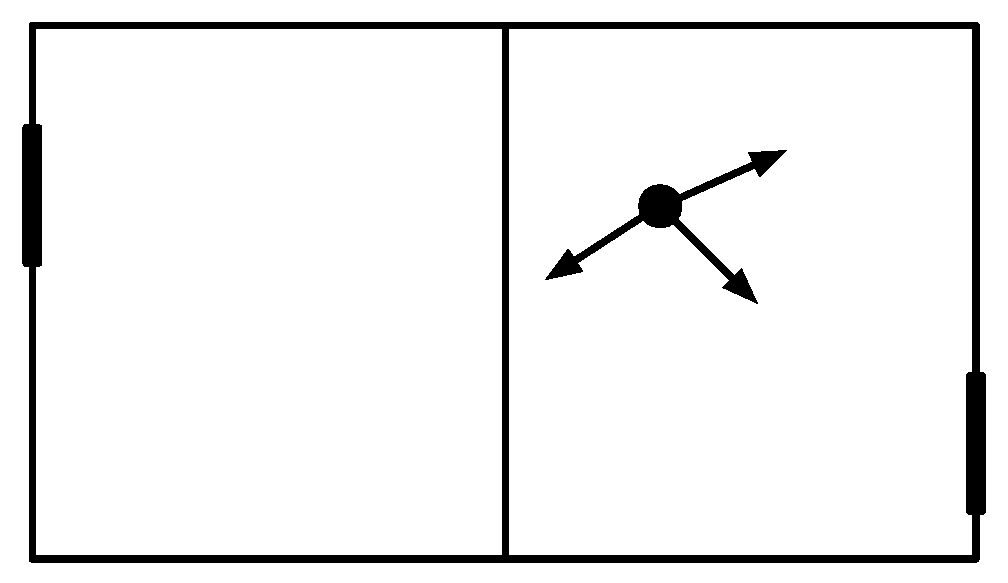
\includegraphics[width=0.90\paperwidth]{recurent.pdf}
    \end{beamercolorbox}%
}


\frame[t]
{
    \frametitle{unser rekurentes Netz}
    
    \begin{beamercolorbox}[center]{}
        %\includegraphics[width=0.90\paperwidth]{recurentNET.pdf}
    \end{beamercolorbox}%
    TODO: hier folgt noch eine Grafik mit dem aufbau eines Rekurenten Netzes
}




\section{zeitverz"ogerte Bewertung} %Fehlerkalkulation
\frame[t]
{
    \frametitle{zeitverz"ogerte Bewertung}
        \begin{beamercolorbox}[center]{}
        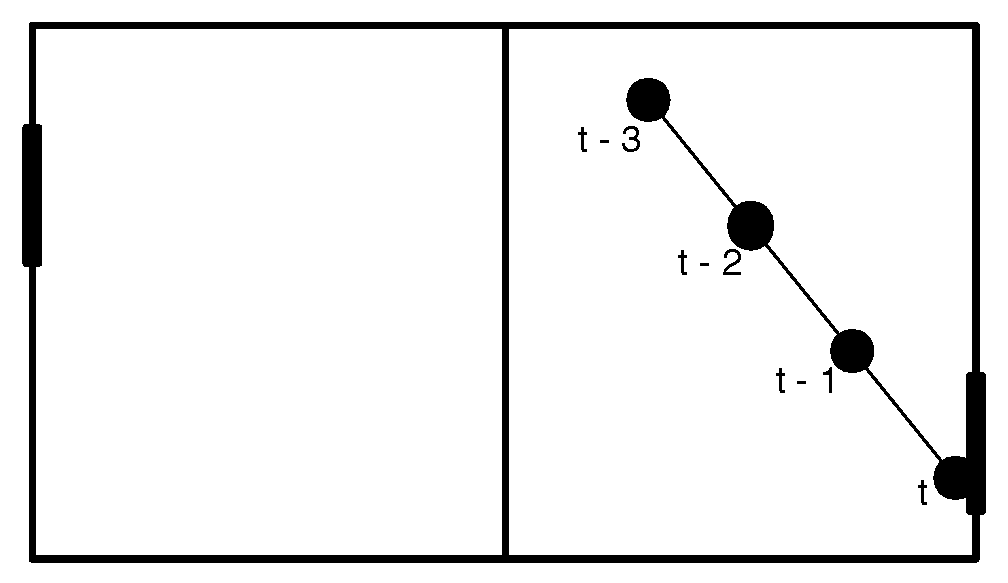
\includegraphics[width=0.9\paperwidth]{delayed.pdf}
    \end{beamercolorbox}%
}

\frame[t]
{
    \frametitle{zeitverz"ogerte Bewertung}
        \begin{beamercolorbox}[center]{}
        %\includegraphics[width=0.9\paperwidth]{delayedFB.pdf}
    \end{beamercolorbox}%
    
    TODO: Hier folgt noch eine Grafik mit dem rekurenten lernen 
}





\section{Demonstration}
\frame[t]
{
  \frametitle{Demonstration}
    \begin{itemize}
        \item nicht trainiertes KNN
        \item trainiertes KNN
    \end{itemize}
  
  TODO: Video oder Live

}

\frame[t]
{
  \frametitle{KNNs gegen"ubergestellt}
  
  TODO: Hier folgt noch eine BALKENDIAGRAMM - GRAFIK mit Vergleich von verschiendenen Konfigurationen. Welches KNN lernt am schnellsten / besten?
  
  %Config -> 1k Iterationen -> 10k Iterationen -> 100k -> 10 Mio
  %xx -> 0.3
  
  %Balkendiagramm

}



\section{Fazit} 

\frame[t]
{
\frametitle{Fazit}
    \begin{itemize}
        \item zeitliche Verz"ogerung
         \item allg. Debugging von KNN
        \item vorverarbeitete Inputdaten
        \item KNN kennt keine physkalischen Gesetze
    \end{itemize}
}

%%%%%%%%%%%%%%

\frame[c]{
  \frametitle{The End}
\begin{center}
  Danke f"ur Ihre Aufmerksamkeit.\\[1ex]
  Weitere Fragen?\\[5ex]
\end{center}
}

\end{document}
